\subsubsection{Multi-Directional Bearing Angle Image}

The \emph{\gls{multi-directional-bearing-angle-image}} attempts to overcome the limitation of missing rotation invariance for the classical \gls{bearing-angle-image}.
Instead of computing one angle in one direction, the two adjacent triangle are combined.
Figure~\ref{fig:max-curve} shows how the triangles are related.
Both angles $\beta$ and $\gamma$ are calculated with Equation~\ref{eq:bearing-angle}.
For $\gamma$ the values of $d_{i,j}$ and $d_{i-1,j}$ need to be swapped.
\begin{figure}
    \scalebox{0.9}{%
    

\tikzset{every picture/.style={line width=0.75pt}} %set default line width to 0.75pt        

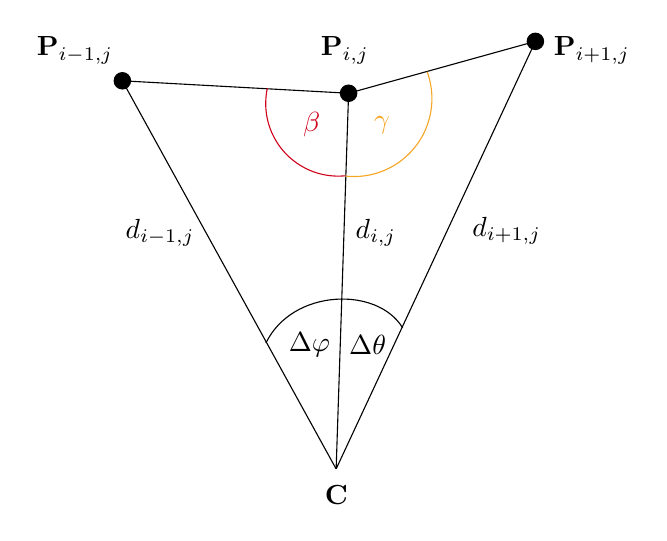
\begin{tikzpicture}[x=0.75pt,y=0.75pt,yscale=-1,xscale=1]
%uncomment if require: \path (0,252); %set diagram left start at 0, and has height of 252

%Straight Lines [id:da05017383740499093] 
\draw    (46.83,26.67) -- (149.83,213.67) ;
%Straight Lines [id:da6895513561877372] 
\draw    (155.83,32.67) -- (149.83,213.67) ;
%Curve Lines [id:da10253757735662583] 
\draw [color={rgb, 255:red, 0; green, 0; blue, 0 }  ,draw opacity=1 ]   (116,153) .. controls (128.83,126.67) and (169.83,125.67) .. (181.83,145.67) ;
%Straight Lines [id:da3851492122035306] 
\draw    (46.83,26.67) -- (155.83,32.67) ;
%Shape: Circle [id:dp08101382020617043] 
\draw  [fill={rgb, 255:red, 0; green, 0; blue, 0 }  ,fill opacity=1 ] (151.88,32.67) .. controls (151.88,30.49) and (153.65,28.72) .. (155.83,28.72) .. controls (158.01,28.72) and (159.78,30.49) .. (159.78,32.67) .. controls (159.78,34.85) and (158.01,36.62) .. (155.83,36.62) .. controls (153.65,36.62) and (151.88,34.85) .. (151.88,32.67) -- cycle ;
%Shape: Circle [id:dp7397482298206297] 
\draw  [fill={rgb, 255:red, 0; green, 0; blue, 0 }  ,fill opacity=1 ] (42.88,26.67) .. controls (42.88,24.49) and (44.65,22.72) .. (46.83,22.72) .. controls (49.01,22.72) and (50.78,24.49) .. (50.78,26.67) .. controls (50.78,28.85) and (49.01,30.62) .. (46.83,30.62) .. controls (44.65,30.62) and (42.88,28.85) .. (42.88,26.67) -- cycle ;
%Shape: Circle [id:dp7936487176657823] 
\draw  [fill={rgb, 255:red, 0; green, 0; blue, 0 }  ,fill opacity=1 ] (241.88,7.67) .. controls (241.88,5.49) and (243.65,3.72) .. (245.83,3.72) .. controls (248.01,3.72) and (249.78,5.49) .. (249.78,7.67) .. controls (249.78,9.85) and (248.01,11.62) .. (245.83,11.62) .. controls (243.65,11.62) and (241.88,9.85) .. (241.88,7.67) -- cycle ;
%Straight Lines [id:da7225304487809803] 
\draw    (245.83,7.67) -- (149.83,213.67) ;
%Straight Lines [id:da15289701870660388] 
\draw    (155.83,32.67) -- (245.83,7.67) ;
%Shape: Arc [id:dp845909277560968] 
\draw  [draw opacity=0] (154.29,72.43) .. controls (153.16,72.54) and (152.02,72.6) .. (150.87,72.6) .. controls (131.56,72.6) and (115.9,56.94) .. (115.9,37.63) .. controls (115.9,35.08) and (116.17,32.59) .. (116.69,30.19) -- (150.87,37.63) -- cycle ; \draw  [color={rgb, 255:red, 208; green, 2; blue, 27 }  ,draw opacity=1 ] (154.29,72.43) .. controls (153.16,72.54) and (152.02,72.6) .. (150.87,72.6) .. controls (131.56,72.6) and (115.9,56.94) .. (115.9,37.63) .. controls (115.9,35.08) and (116.17,32.59) .. (116.69,30.19) ;
%Shape: Arc [id:dp15343497156889918] 
\draw  [draw opacity=0] (193.67,22.29) .. controls (195.16,26.33) and (195.97,30.7) .. (195.97,35.25) .. controls (195.97,55.99) and (179.15,72.8) .. (158.42,72.8) .. controls (157.06,72.8) and (155.72,72.73) .. (154.4,72.59) -- (158.42,35.25) -- cycle ; \draw  [color={rgb, 255:red, 245; green, 166; blue, 35 }  ,draw opacity=1 ] (193.67,22.29) .. controls (195.16,26.33) and (195.97,30.7) .. (195.97,35.25) .. controls (195.97,55.99) and (179.15,72.8) .. (158.42,72.8) .. controls (157.06,72.8) and (155.72,72.73) .. (154.4,72.59) ;

% Text Node
\draw (137,154) node  [color={rgb, 255:red, 0; green, 0; blue, 0 }  ,opacity=1 ] [align=left] {$\displaystyle \Delta $$\displaystyle \varphi $};
% Text Node
\draw (138,48) node  [color={rgb, 255:red, 208; green, 2; blue, 27 }  ,opacity=1 ] [align=left] {$\displaystyle \beta $};
% Text Node
\draw (169,100) node   [align=left] {$\displaystyle d_{i,j}$};
% Text Node
\draw (65,100) node   [align=left] {$\displaystyle d_{i-1,j}$};
% Text Node
\draw (154,12) node   [align=left] {$\displaystyle \mathbf{P}_{i,j}$};
% Text Node
\draw (150,226) node   [align=left] {$\displaystyle \mathbf{C}$};
% Text Node
\draw (232,99) node   [align=left] {$\displaystyle d_{i+1,j}$};
% Text Node
\draw (172,48) node   [align=left] {$\displaystyle \textcolor[rgb]{0.96,0.65,0.14}{\gamma }$};
% Text Node
\draw (165,154) node  [color={rgb, 255:red, 0; green, 0; blue, 0 }  ,opacity=1 ] [align=left] {$\displaystyle \Delta $$\displaystyle \theta $};
% Text Node
\draw (273,12) node   [align=left] {$\displaystyle \mathbf{P}_{i+1,j}$};
% Text Node
\draw (24,12) node   [align=left] {$\displaystyle \mathbf{P}_{i-1,j}$};


\end{tikzpicture}


    }
    \caption[Schematic representation of the \gls{multi-directional-bearing-angle-image}]{\emph{Schematic representation of the \gls{multi-directional-bearing-angle-image}.} The \gls{multi-directional-bearing-angle-image} composes two \Glspl{bearing-angle} in vertical, horizontal, diagonal and antidiagonal direction. The maximum angle is then selected as pixel value.}\label{fig:max-curve}
\end{figure}
Both angles are added together, resulting in the angle of the surface at this position.
\begin{equation}
    \mathcal{B_{\textit{direction}}}= \beta + \gamma
\end{equation}
This calculation is again only in one direction and not rotation invariant but already symmetrical.
The value $\mathcal{B_{\textit{direction}}}$ can be defined for diagonal, antidiagonal, horizontal and vertical sampling of the image.
The final step for rotation invariance is the reduction of these four values to their maximum:
\vspace{-2mm}
\begin{align}
    \mathcal{B} &= \max{\{\mathcal{B}_{diagonal}, \mathcal{B}_{antidiagonal}, \mathcal{B}_{horizontal}, \mathcal{B}_{vertical}\}}
\end{align}
The converted images in Figure~\ref{fig:max-curve-images} show the same scene and positions as for the \gls{bearing-angle-image}.
\begin{figure}[H]
    \begin{subfigure}[t]{0.32\textwidth}
        
\includegraphics[width=\linewidth]{chapter04/img/max-0001.png}
    \end{subfigure}
    \begin{subfigure}[t]{0.32\textwidth}
        
\includegraphics[width=\linewidth]{chapter04/img/max-0030.png}
    \end{subfigure}
    \begin{subfigure}[t]{0.32\textwidth}
        
\includegraphics[width=\linewidth]{chapter04/img/max-0210.png}
    \end{subfigure}
    \caption[Rotation invariance of \gls{multi-directional-bearing-angle-image}]{\emph{Rotation invariance of \gls{multi-directional-bearing-angle-image}.} The images show the same camera positions as the \gls{bearing-angle} and demonstrates the rotation invariance. Each edge in the geometry forms a visible white line. No other textures exist.}\label{fig:max-curve-images}
\end{figure}
\vspace{-5mm}
The goal of rotational invariance is achieved, unfortunatly the image lacks texture and contrast.
Qualitative tests with common feature detectors yielded weak keypoint responses.
Therefore, this approach received no further attention.
